\documentclass[11pt]{article}
\usepackage[margin=1in]{geometry}
\usepackage{amsmath,amssymb,amsthm,mathtools}
\usepackage{booktabs}
\usepackage{hyperref}
\usepackage{tikz}
\usetikzlibrary{arrows.meta,positioning}

\title{Convex Pattern Amplification Under Deletion\\\large A deterministic selection principle for U-statistics and induced substructure laws}
\author{Sven Hardy Benson}
\date{12 September 2026}

\newtheorem{theorem}{Theorem}
\newtheorem{corollary}{Corollary}
\newtheorem{lemma}{Lemma}
\newtheorem{remark}{Remark}

\newcommand{\E}{\mathbb E}
\newcommand{\R}{\mathbb R}
\newcommand{\KL}{D_{\mathrm{KL}}}

\begin{document}
\maketitle

\begin{abstract}
Let $V$ be finite. For each $j=1,\dots,d$, choose an order $r_j$ and a real kernel on the $r_j$-subsets of $V$. For every sufficiently large $S\subseteq V$, let $U(S)\in\R^d$ be the vector of normalized U-statistics. The exact deletion identity
\[
U(S)=\frac1{|S|}\sum_{v\in S}U(S\setminus\{v\})
\]
places the parent profile at the barycenter of its one-point deletion profiles. Jensen's inequality then implies that for every convex $\Phi:\R^d\to\R$ some deletion satisfies
\[
\Phi(U(S\setminus\{v\}))\ge \Phi(U(S)).
\]
Iteration produces a deterministic nested chain of induced substructures along which $\Phi$ never decreases. For quadratic potentials the mean gain is exactly the leave-one-out variance of the deletion profiles. Applied to induced graph-pattern laws, the principle yields nested induced subgraphs with nondecreasing collision energy and Kullback--Leibler divergence from a fixed positive reference law, and nonincreasing Shannon entropy.
\end{abstract}

\section{Setup}
Let $V$ be finite. Fix $d\ge1$. For every $j$ choose $r_j\ge1$ and
\[
h_j:\binom{V}{r_j}\to\R.
\]
Let $r_*:=\max_j r_j$. For $S\subseteq V$ with $|S|\ge r_*$ define
\[
U_j(S)=\binom{|S|}{r_j}^{-1}\sum_{A\in\binom{S}{r_j}}h_j(A),
\qquad
U(S)=(U_1(S),\dots,U_d(S)).
\]

\section{Deletion barycenter}
\begin{theorem}[Exact deletion barycenter]
If $|S|>r_*$, then
\[
U(S)=\frac1{|S|}\sum_{v\in S}U(S\setminus\{v\}).
\]
\end{theorem}

\begin{proof}
Fix $j$ and put $r=r_j$, $m=|S|$. Expanding the deletion sum gives
\[
\sum_{v\in S}U_j(S\setminus\{v\})
=\binom{m-1}{r}^{-1}
\sum_{v\in S}\sum_{A\in\binom{S\setminus\{v\}}r}h_j(A).
\]
Every fixed $A\in\binom Sr$ survives precisely the $m-r$ deletions with $v\notin A$. Hence the double sum equals
\[
(m-r)\sum_{A\in\binom Sr}h_j(A).
\]
Using
\[
\binom{m-1}{r}=\frac{m-r}{m}\binom mr
\]
we obtain
\[
\sum_{v\in S}U_j(S\setminus\{v\})=mU_j(S).
\]
Divide by $m$ and repeat for each coordinate.
\end{proof}

\begin{figure}[ht]
\centering
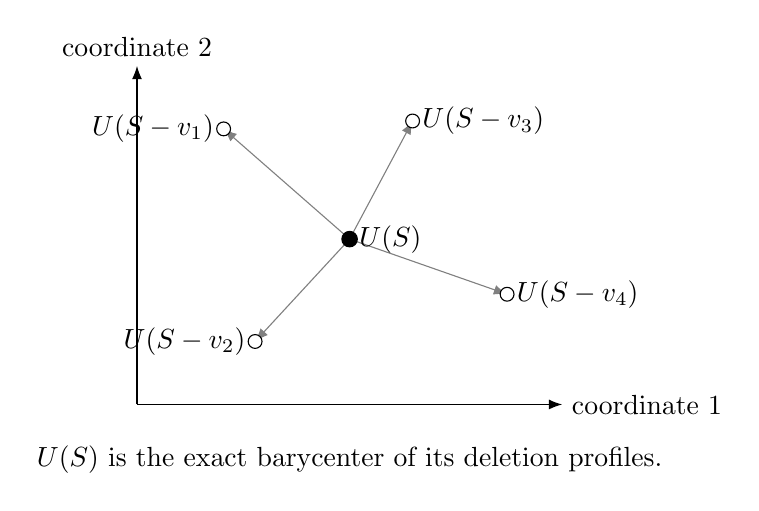
\begin{tikzpicture}[scale=1.0,>=Latex]
  \draw[->] (0,0) -- (5.4,0) node[right] {coordinate 1};
  \draw[->] (0,0) -- (0,4.3) node[above] {coordinate 2};
  \coordinate (p) at (2.7,2.1);
  \coordinate (a) at (1.1,3.5);
  \coordinate (b) at (1.5,0.8);
  \coordinate (c) at (3.5,3.6);
  \coordinate (d) at (4.7,1.4);
  \foreach \x in {a,b,c,d} {\draw[->,gray] (p) -- (\x); \filldraw[fill=white] (\x) circle (2.5pt);}
  \fill (p) circle (3pt);
  \node[right] at (p) {$U(S)$};
  \node[left] at (a) {$U(S-v_1)$};
  \node[left] at (b) {$U(S-v_2)$};
  \node[right] at (c) {$U(S-v_3)$};
  \node[right] at (d) {$U(S-v_4)$};
  \node at (2.7,-0.7) {$U(S)$ is the exact barycenter of its deletion profiles.};
\end{tikzpicture}
\caption{The finite identity driving the selection theorem.}
\end{figure}

\section{Convex amplification}
\begin{theorem}[One-step convex amplification]
Let $\Phi:\R^d\to\R$ be convex. If $|S|>r_*$, then some $v\in S$ satisfies
\[
\Phi(U(S\setminus\{v\}))\ge \Phi(U(S)).
\]
\end{theorem}

\begin{proof}
By the deletion barycenter identity and Jensen,
\[
\Phi(U(S))
=\Phi\left(\frac1{|S|}\sum_{v\in S}U(S\setminus\{v\})\right)
\le \frac1{|S|}\sum_{v\in S}\Phi(U(S\setminus\{v\})).
\]
At least one summand is no smaller than the average.
\end{proof}

\begin{corollary}[Nested amplification chain]
For every $m$ with $r_*\le m\le|V|$, there is a chain
\[
V=S_n\supset S_{n-1}\supset\cdots\supset S_m,
\qquad |S_t|=t,
\]
such that
\[
\Phi(U(S_n))\le\Phi(U(S_{n-1}))\le\cdots\le\Phi(U(S_m)).
\]
\end{corollary}

\begin{proof}
Apply the one-step theorem recursively.
\end{proof}

If $\Phi$ is strictly convex and the deletion profiles are not all equal, Jensen is strict, so some deletion strictly increases $\Phi$.

\section{Quadratic gain and jackknife variance}
Fix $c\in\R^d$ and define
\[
E_c(S)=\|U(S)-c\|_2^2
\]
and
\[
J(S)=\frac1{|S|}\sum_{v\in S}
\|U(S\setminus\{v\})-U(S)\|_2^2.
\]

\begin{theorem}[Exact quadratic energy accounting]
If $|S|>r_*$, then
\[
\frac1{|S|}\sum_{v\in S}E_c(S\setminus\{v\})=E_c(S)+J(S).
\]
Consequently some deletion has
\[
E_c(S\setminus\{v\})\ge E_c(S)+J(S).
\]
\end{theorem}

\begin{proof}
Write $x_v=U(S\setminus\{v\})$ and $\bar x=U(S)$. The deletion identity gives $\bar x=|S|^{-1}\sum_v x_v$. Expand
\[
\|x_v-c\|^2
=\|x_v-\bar x\|^2+\|\bar x-c\|^2
+2\langle x_v-\bar x,\bar x-c\rangle.
\]
The cross terms vanish after averaging because $\sum_v(x_v-\bar x)=0$.
\end{proof}

Choosing at each stage a child whose energy gain is at least the current average yields
\[
E_c(S_m)\ge E_c(V)+\sum_{t=m+1}^{n}J(S_t).
\]
Thus the selected chain converts leave-one-out instability into deterministic structural amplification.

\section{Induced graph-pattern laws}
Let $G$ be a finite simple graph and fix $r\ge2$. Let $\mathcal G_r$ denote the unlabeled graphs on $r$ vertices. For $H\in\mathcal G_r$ set
\[
p_H(S)=\frac{\#\{A\in\binom Sr:G[A]\cong H\}}{\binom{|S|}{r}}.
\]
The vector $p_r(S)=(p_H(S))_{H\in\mathcal G_r}$ is a probability distribution and satisfies the deletion barycenter identity.

\begin{corollary}[Collision energy]
There is a nested induced chain along which
\[
C_r(S):=\sum_H p_H(S)^2
\]
is nondecreasing.
\end{corollary}

\begin{corollary}[Entropy descent]
There is a nested induced chain along which
\[
\mathsf H_r(S):=-\sum_H p_H(S)\log p_H(S)
\]
is nonincreasing.
\end{corollary}

\begin{corollary}[KL amplification]
Fix a probability law $q=(q_H)_H$ with every $q_H>0$. There is a nested induced chain along which
\[
\KL(p_r(S)\|q)=\sum_H p_H(S)\log\frac{p_H(S)}{q_H}
\]
is nondecreasing.
\end{corollary}

For $0<p<1$, one may choose $q$ to be the unlabeled $r$-vertex law of the Erd\H{o}s--R\'enyi graph $G(r,p)$.

\section{Computational check}
The companion Python script exhaustively enumerates all
\[
2^{\binom 62}=32768
\]
labeled graphs on six vertices. For every graph it verifies the deletion barycenter identity for edge and triangle density and checks that a greedy quadratic-energy deletion never decreases the potential.

A deterministic 14-vertex example uses the full three-vertex pattern law, classified by edge count $0,1,2,3$. Against
\[
q=(1/8,3/8,3/8,1/8),
\]
the $G(3,1/2)$ reference law, the greedy KL chain gives:

\begin{center}
\begin{tabular}{rr}
\toprule
Vertices & $D_{\mathrm{KL}}$ \\
\midrule
14 & 0.04592\\
13 & 0.12483\\
12 & 0.24643\\
11 & 0.38320\\
10 & 0.58679\\
9  & 0.87787\\
8  & 1.09837\\
7  & 1.16728\\
6  & 1.35932\\
5  & 2.07944\\
\bottomrule
\end{tabular}
\end{center}

These computations are a falsification harness, not a substitute for proof.

\section{Prior art and novelty posture}
U-statistics were introduced by Hoeffding in 1948 \cite{hoeffding1948}. Their reverse-martingale structure is classical; Christofides and Serfling exploit it for generalized U-statistics \cite{christofides1990}. Sampling and local pattern densities are foundational in graph-limit theory \cite{lovasz2012}, and pattern-density vectors are central in flag algebras \cite{razborov2007}. Induced-subgraph density remains an active structural theme; see, for example, Nguyen, Scott and Seymour \cite{nguyen2026}.

The present note does not claim those ingredients as new. The targeted search for this draft did not locate the exact package consisting of a simultaneous multi-order vector profile, arbitrary convex potential, recursively nested deterministic deletion chain, exact quadratic gain identity, and the induced-pattern entropy/KL corollaries. That is a provisional literature finding, not proof of priority.

\section{Formalization boundary}
The pinned Lean project in \texttt{papers/code/convex\_pattern\_amplification/} formalizes the abstract finite barycenter-selection spine and a scalar quadratic variance identity. The full graph-pattern encoding and the kernel double-counting theorem remain ordinary mathematical proofs in this draft. The Lean source contains no \texttt{sorry}, \texttt{admit}, or user-declared \texttt{axiom}; the current authoring environment lacks Lean/Lake, so the status is \emph{formalized, compiler check pending}.

\begin{thebibliography}{9}
\bibitem{hoeffding1948}
W. Hoeffding,
\emph{A Class of Statistics with Asymptotically Normal Distribution},
Annals of Mathematical Statistics 19 (1948), 293--325.
\href{https://doi.org/10.1214/aoms/1177730196}{doi:10.1214/aoms/1177730196}.

\bibitem{christofides1990}
T. C. Christofides and R. J. Serfling,
\emph{Maximal inequalities and convergence results for generalized U-statistics},
Journal of Statistical Planning and Inference 24 (1990), 271--286.
\href{https://doi.org/10.1016/0378-3758(90)90048-Y}{doi:10.1016/0378-3758(90)90048-Y}.

\bibitem{lovasz2012}
L. Lov\'asz,
\emph{Large Networks and Graph Limits},
AMS Colloquium Publications 60, 2012.
\href{https://doi.org/10.1090/coll/060}{doi:10.1090/coll/060}.

\bibitem{razborov2007}
A. A. Razborov,
\emph{Flag Algebras},
Journal of Symbolic Logic 72 (2007), 1239--1282.
\href{https://doi.org/10.2178/jsl/1203350785}{doi:10.2178/jsl/1203350785}.

\bibitem{nguyen2026}
T. Nguyen, A. Scott and P. Seymour,
\emph{Induced subgraph density. VII. The five-vertex path},
Proceedings of the London Mathematical Society 132 (2026).
\href{https://doi.org/10.1112/plms.70133}{doi:10.1112/plms.70133}.
\end{thebibliography}

\end{document}
